\documentclass{article}
\usepackage{tikz}
\usetikzlibrary{arrows.meta}

\begin{document}

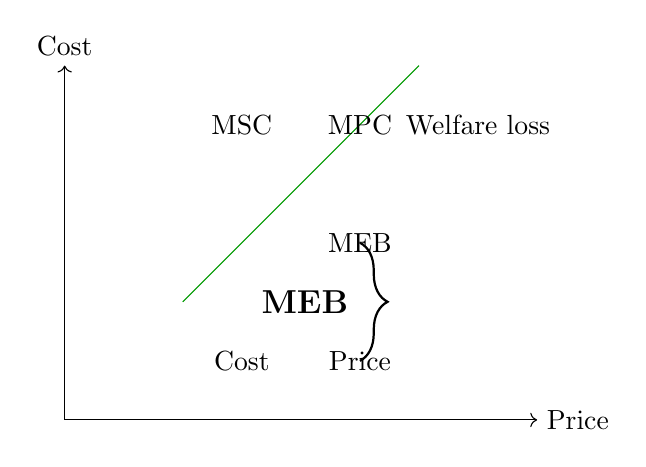
\begin{tikzpicture}[scale=1.5]
    % Draw the axes
    \draw[->] (0,0) -- (4,0) node[right] {Price};
    \draw[->] (0,0) -- (0,3) node[above] {Cost};

    % Draw the green triangle for positive consumption externality
    \filldraw[green!60!black] (2,2) -- (3,3) -- (1,1) -- cycle;

    % Label the terms
    \node at (3.5, 2.5) {Welfare loss};
    \node at (2.5, 2.5) {MPC};
    \node at (1.5, 2.5) {MSC};
    \node at (2.5, 1.5) {MEB};
    \node at (2.5, 0.5) {Price};
    \node at (1.5, 0.5) {Cost};

    % Add a curly brace around MEB
    \draw[decorate, decoration={brace, amplitude=10pt}, thick] (2.5, 1.5) -- (2.5, 0.5) node [black,midway,xshift=-0.7cm] {\textbf{\large MEB}};

\end{tikzpicture}

\end{document}